\question Q2\droppoints

\begin{solution}
    \text{(a) - (d)} Implemented.

    \text{(e)}

    \centerline {
        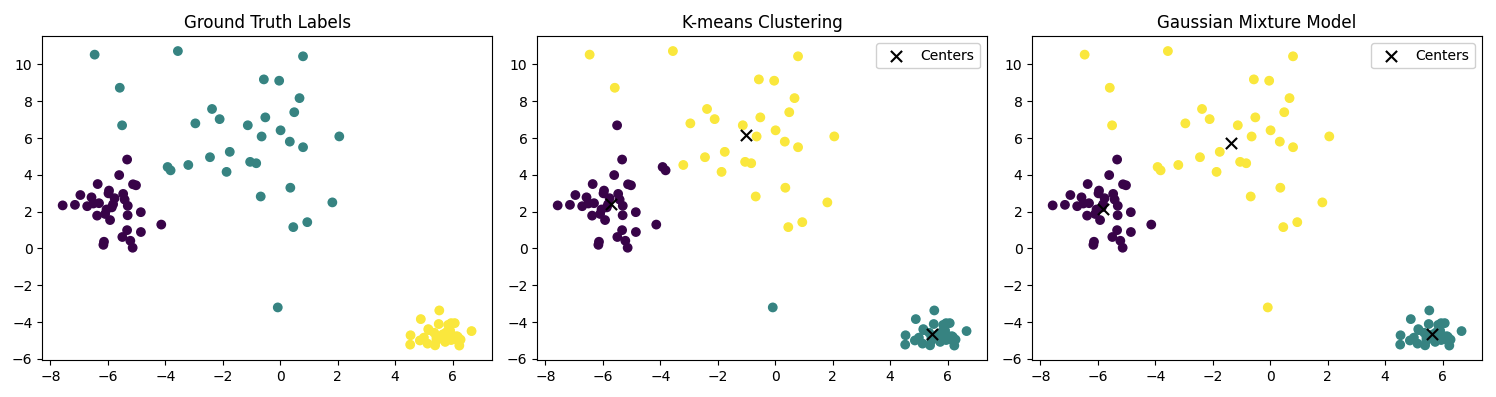
\includegraphics[width=\textwidth]{img/blob_comparison}
    }

    \text{(f)}

    \centerline {
        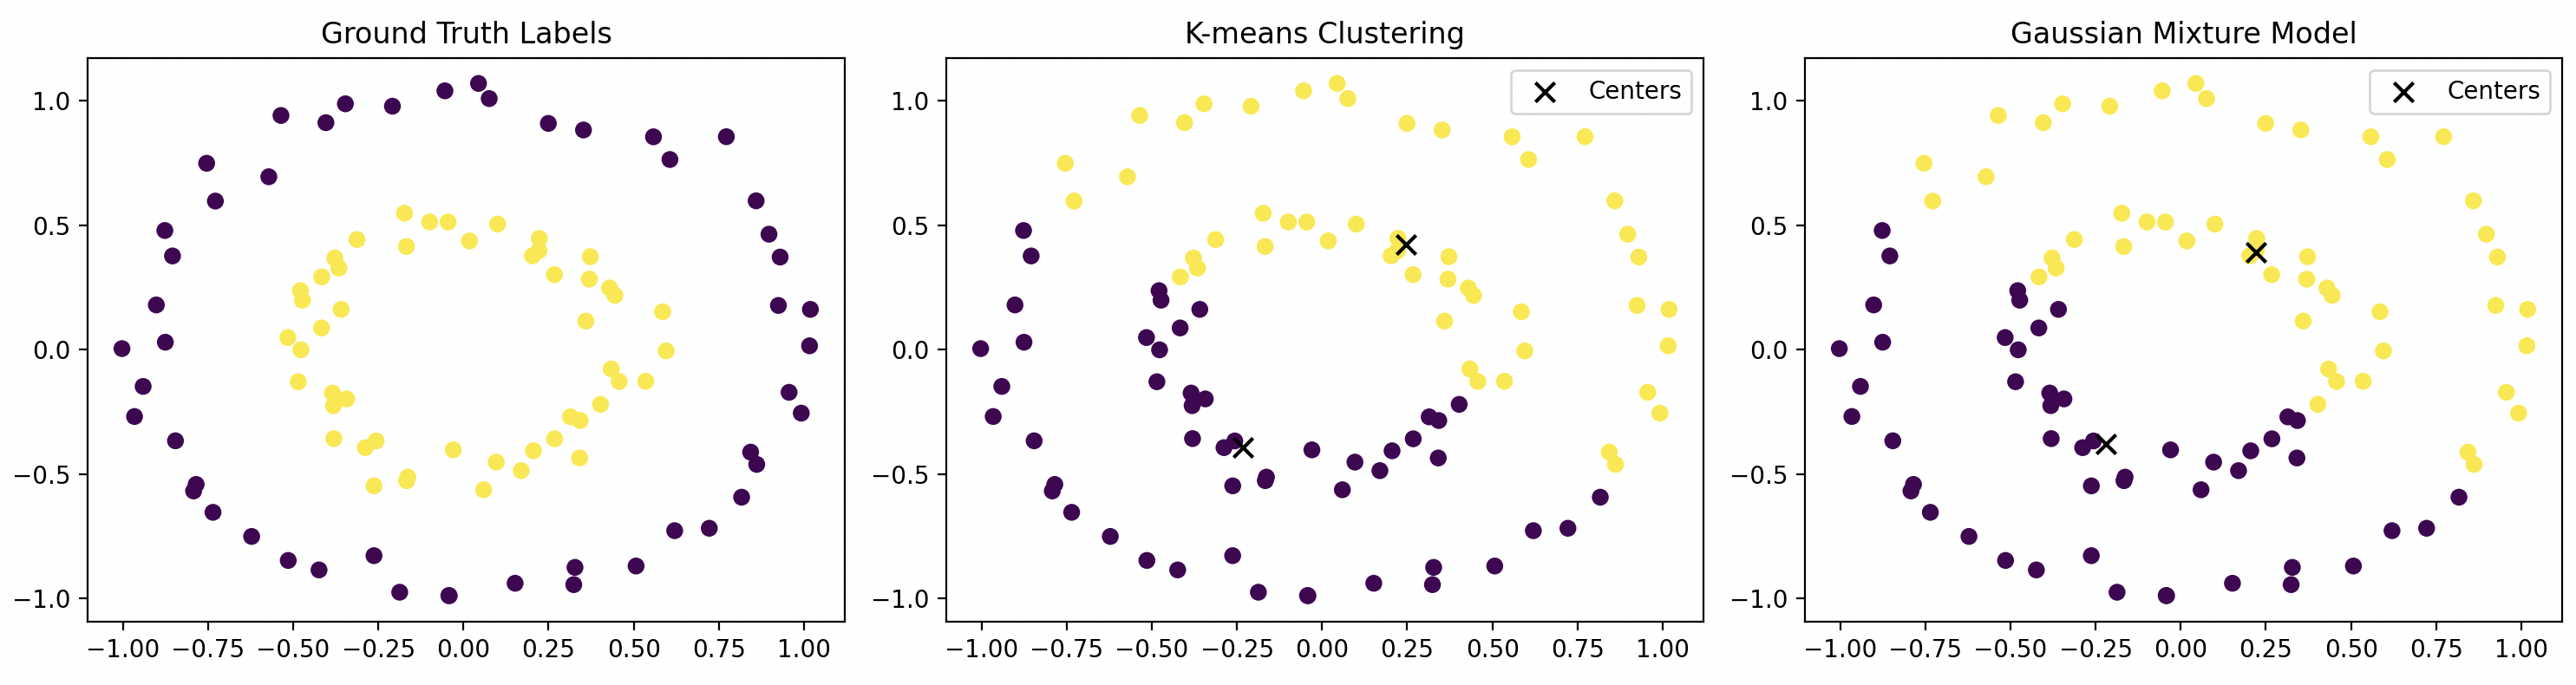
\includegraphics[width=\textwidth]{img/circle_comparison}
    }

    \text{(g)}

    \centerline {
        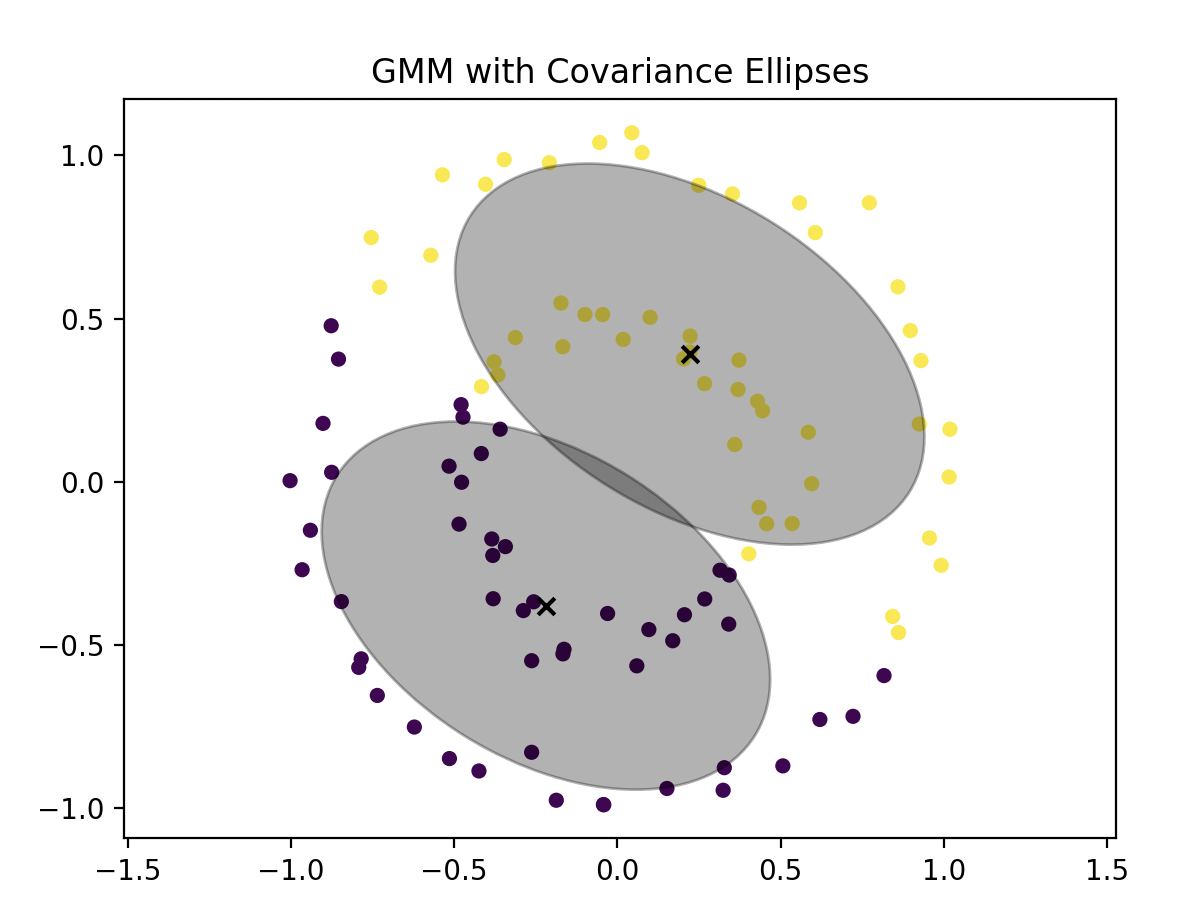
\includegraphics[width=0.8\textwidth]{img/covariance_ellipses}
    }

    \text{(h)} I used the \textbf{adjusted\_rand\_score} function to measures the similarity of the two assignments, ignoring permutations.
    The result table is as follows:

    \begin{center}
        \begin{tabular}{ c c c }
            \hline
            ${ }$   & $D_{\text{blob}}$ & $D_{\text{circle}}$ \\
            \hline
            K-means & 0.8837            & -0.0132             \\
            GMM     & 1.0000            & -0.0132             \\
            \hline
        \end{tabular}
    \end{center}

    We can see that for the Blob database, the Adjusted Rand Score (ARS) is pretty high for both K-Means and GMM, meaning that both models perform well on this dataset.

    However, both K-Means and GMM perform very bad on the Circle dataset.
    Both ARSs are negative and close to zero, which means the clustering is no better than random.
    This is because the two algorithms assume that clusters are elliptical or spherical in nature.
    But the Circle dataset is in ring-shaped, which violates the assumption.
    The \textbf{DBSCAN Clustering} model fits this dataset better.

    \text{(i)} The default method that is used to initialize cluster centers in GMM is \textbf{kmeans}.

    \begin{center}
        \begin{tabular}{ c c }
            \hline
            \#  & Score   \\
            \hline
            1   & 0.0476  \\
            2   & -0.0119 \\
            3   & 0.1286  \\
            4   & 0.0076  \\
            5   & -0.0083 \\
            \hline
            AVG & 0.0327  \\
            \hline
        \end{tabular}
    \end{center}

    While GMM with random initial parameters has a higher average score, it still doesn't fit the \textbf{make\_circles} dataset.
    The reason they performance better than \textbf{k-means} is random initialization explores more of the parameter space, while K-Means is more deterministic and stable.

    \text{(j)} In clustering problems, choosing a proper clustering method is significant.
    In \url{https://scikit-learn.org/stable/modules/clustering.html}, there lists a variety of dataset types and the visual performances of using different clustering methods.
    When it comes to the ring-shaped dataset we have in \textbf{make\_circles}, DBSCAN Clustering turns out to be a good option.
    I have implemented it in the Python file.
    The resulting image is as follows:

    \centerline {
        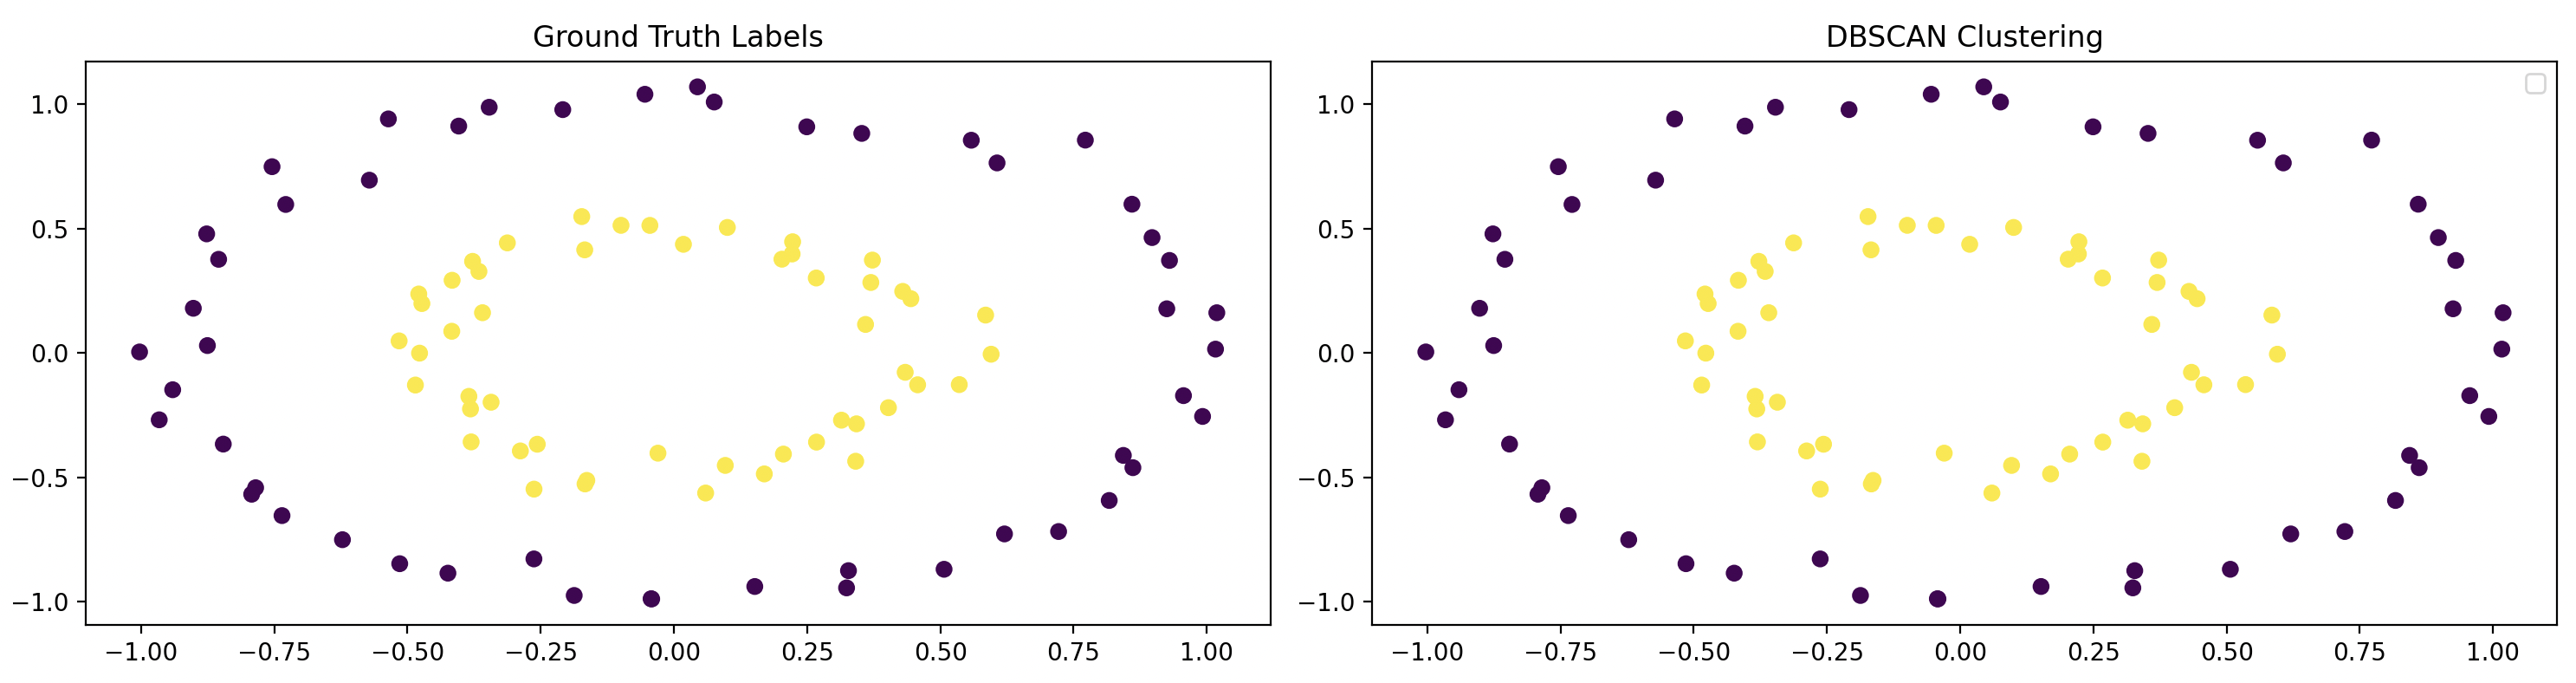
\includegraphics[width=1.0\textwidth]{img/dbscan}
    }
\end{solution}